Every chapter so far assumes access to a scalar reward signal: dynamic programming requires $r(s,a)$, model-free RL observes $r_t$ after each transition, and the Bellman optimality equation presupposes that rewards are known or observable. When they are neither, the DP/RL machinery cannot be applied directly.

In many domains, scalar rewards are unavailable but ordinal preferences over trajectories are easy to elicit. A human evaluator cannot assign a meaningful numerical score to a paragraph of text, but can reliably say ``response A is better than response B.'' The raw data is a set of trajectory pairs with binary preference labels. Reinforcement learning from human feedback (RLHF) uses these ordinal comparisons to learn a proxy reward function $r_\theta$, which then serves as the scalar signal for standard RL optimization. This is not an inverse problem in the IRL sense; the goal is not to rationalize observed behavior, but rather a two-stage forward problem in which the analyst first learns a reward from human judgments and then solves the resulting MDP. \citet{christiano:2017} demonstrated that this approach could train agents without an explicit reward function. RLHF has since become the predominant method for aligning large language models.

\subsection{Learning Rewards from Preferences}

The canonical RLHF framework is built on a formal model of human preference. The observed data consists of tuples $(s, y_w, y_l)$, where $s$ is a context, and $y_w$ and $y_l$ are two outputs, with $y_w$ being the ``winner'' preferred by a human. Assuming preferences follow a latent utility model, the Bradley-Terry model \citep{bradley1952rank} gives the probability that $y_w$ is preferred: $P(y_w \succ y_l | s) = \sigma(r_\theta(s, y_w) - r_\theta(s, y_l))$, where $r_\theta: \mathcal{S} \times \mathcal{Y} \to \mathbb{R}$ is a learned \textit{reward model} parameterized by $\theta$, trained to approximate human preferences (not the ground-truth reward, which is unobserved), and $\sigma(\cdot)$ is the logistic function. This formulation is a binary logit model (Section~\ref{section:language}, Equation~\ref{eq:softmax_logit}).\footnote{\citet{iskhakov2021} discuss the contrasts and synergies between machine learning and structural econometrics, including the shared reliance on logit-based choice models that underlies both RLHF and dynamic discrete choice estimation.} The reward model parameters $\theta$ are estimated by minimizing the negative log-likelihood of the observed human choices:
\begin{equation}
    \mathcal{L}(\theta) = -\mathbb{E}_{(s, y_w, y_l) \sim \mathcal{D}} \left[ \log \sigma \left( r_\theta(s, y_w) - r_\theta(s, y_l) \right) \right],
\label{eq:rlhf_loss}
\end{equation}
In the LLM setting, the ``outputs'' $y_w$ and $y_l$ are token sequences, i.e., trajectories of the autoregressive policy\footnote{An \emph{autoregressive} language model generates text token by token: at each step it outputs a distribution over the vocabulary conditioned on all preceding tokens, then samples the next token; the full response is therefore a trajectory in token space and the model acts as a sequential policy over a vocabulary-sized action set.}, so preferences are over trajectories rather than single actions. The preference loss in Equation~(\ref{eq:rlhf_loss}) is MLE of a choice model where the ``alternatives'' are trajectory segments and the ``choice'' is the human-preferred one.

This logit foundation is also a social-choice assumption once labelers are heterogeneous. Pooling pairwise comparisons from many evaluators does not recover a neutral ``human preference''; it estimates a single score whose odds ratios summarize the aggregation rule induced by the sampling scheme, label model, and loss function. Recent alignment work makes this point explicit: standard Bradley-Terry-style reward learning can behave like a hidden social welfare function, can fail natural axioms for aggregating rankings, and can create strategic reporting incentives when preferences differ across contexts or groups \citep{conitzer2024socialchoice,siththaranjan2024distributional,ge2024axioms,park2024heterogeneous}. DPO inherits the same aggregation problem because it replaces the explicit reward model with an implicit reward difference, not with a theory of whose preferences count.

\subsection{The RLHF Pipeline and Direct Optimization}

The learned $r_\theta$ then serves as a proxy objective for policy optimization. Building on the reward-learning and RL fine-tuning framework of \citet{ziegler2019fine} and \citet{stiennon2020learning}, the canonical three-stage pipeline was formalized by \citet{ouyang2022training}. First, a base pretrained model is initialized via supervised fine-tuning (SFT)\footnote{\emph{Pretraining} optimizes a language model to predict the next token across a massive text corpus, producing broad linguistic knowledge with no behavioral objective. \emph{Supervised fine-tuning} (SFT) continues training on a small curated dataset of (prompt, ideal-response) pairs to specialize the model toward the desired task and establish the reference policy $\pi^{SFT}$ from which the KL penalty is measured.} on a small dataset of high-quality demonstrations, yielding an initial policy $\pi^{SFT}$. This grounds the model in the desired style and format. The second step is the reward model training as described, using preference data generated from this $\pi^{SFT}$.

In the third step, the SFT policy $\pi_\phi$ is fine-tuned via PPO (Section~\ref{sec:actor_critic}) to maximize the frozen reward model $r_\theta$,\footnote{After fine-tuning concludes, the reward model may be reused for evaluation or for later alignment iterations, but it is not updated inside the PPO optimization loop.} with a KL-divergence penalty preventing the policy from drifting into regions where $r_\theta$ is unreliable. The objective is
\begin{equation}
    J(\phi) = \mathbb{E}_{s \sim \mathcal{D}, y \sim \pi_\phi(\cdot|s)} [r_\theta(s, y)] - \lambda_{KL} \mathbb{E}_{s \sim \mathcal{D}} [D_{KL}(\pi_\phi(\cdot|s) \,||\, \pi^{SFT}(\cdot|s))],
\label{eq:rlhf_objective}
\end{equation}
where $D_{KL}$ is the Kullback-Leibler divergence and $\lambda_{KL}$ controls the penalty strength.\footnote{$\lambda_{KL}$ denotes the KL penalty weight, reserving $\beta$ for model parameters and $\gamma$ for discount factors. The standard RLHF literature, including \citet{rafailov2023direct}, uses $\beta$ for this parameter.} Without this constraint, the policy exploits inaccuracies in $r_\theta$ to achieve high proxy scores with degenerate behavior (``reward hacking''), the RLHF analogue of divergence under function approximation (Section~\ref{sec:deadly_triad}).

The KL-regularized objective in Equation~(\ref{eq:rlhf_objective}) admits a Bayesian interpretation \citep{korbak2022rl}. In this view, the reference policy $\pi^{SFT}$ acts as a prior distribution over plausible responses. The reward model $r_\theta$ provides evidence, specifying which responses are more desirable. The goal of alignment is to find the posterior distribution $\pi^*$ that optimally combines the prior with this evidence. This ideal posterior policy takes the form of Equation~(\ref{eq:rlhf_posterior}):
\begin{equation}
    \pi^*(y|s) \propto \pi^{SFT}(y|s) \exp\left(\frac{r_\theta(s, y)}{\lambda_{KL}}\right).
\label{eq:rlhf_posterior}
\end{equation}
The reward function scaled by $\lambda_{KL}$ defines the log-likelihood, so the KL-regularized objective $J(\phi)$ is equivalent (up to an additive constant) to the Evidence Lower Bound (ELBO) for this Bayesian inference problem. Maximizing the RLHF objective via PPO is therefore variational inference: finding the policy $\pi_\phi$ that minimizes KL divergence to $\pi^*$. This reframes the KL penalty as a structural component of the inference problem rather than an ad-hoc regularizer.

Despite this closed-form characterization, the three-stage RLHF pipeline is complex to implement, requiring training multiple large models and a computationally expensive RL loop. Direct Preference Optimization (DPO), introduced by \citet{rafailov2023direct}, collapses the pipeline into a single supervised learning objective by reparameterizing the reward function in terms of $\pi^*$ and $\pi^{SFT}$, as in Equation~(\ref{eq:dpo_reparameterize}):
\begin{equation}
    r(s,y) = \lambda_{KL} \log\left(\frac{\pi^*(y|s)}{\pi^{SFT}(y|s)}\right) + \lambda_{KL} \log Z(s).
\label{eq:dpo_reparameterize}
\end{equation}
When this analytical expression for the reward is substituted into the Bradley-Terry preference loss from Equation~(\ref{eq:rlhf_loss}), the unknown partition function $Z(s)$ cancels out. This yields a loss function that depends only on the policy $\pi_\phi$ being optimized and the fixed reference policy $\pi^{SFT}$. The DPO objective, given in Equation~(\ref{eq:dpo_loss}), is thus a simple binary cross-entropy loss over policy likelihoods:
\begin{equation}
    \mathcal{L}_{DPO}(\phi; \pi^{SFT}) = -\mathbb{E}_{(s, y_w, y_l) \sim \mathcal{D}} \left[ \log \sigma \left( \lambda_{KL} \log \frac{\pi_\phi(y_w|s)}{\pi^{SFT}(y_w|s)} - \lambda_{KL} \log \frac{\pi_\phi(y_l|s)}{\pi^{SFT}(y_l|s)} \right) \right].
\label{eq:dpo_loss}
\end{equation}
This objective is optimized on $\phi$ using standard supervised learning with a static preference dataset. The gradient increases the likelihood of preferred responses $y_w$ and decreases the likelihood of dispreferred responses $y_l$, relative to the reference policy.

The growing family of DPO variants is best read economically by asking what part of the preference problem changes. IPO modifies the link/objective structure to avoid some DPO overfitting behavior \citep{azar2024preferenceparadigm}. KTO replaces pairwise comparisons with a prospect-theory-style objective over desirable and undesirable outputs \citep{ethayarajh2024kto}. Nash-LHF and SPPO treat preference optimization as a game over pairwise comparisons, which is closer to social choice when preferences are cyclic or non-transitive \citep{munos2023nash,wu2024sppo}. MaxMin-RLHF makes the aggregation rule explicitly egalitarian \citep{chakraborty2024maxmin}. ORPO, SimPO, and robust DPO mainly change implementation, reference-model dependence, or noisy-label bias rather than the underlying welfare question \citep{hong2024orpo,meng2024simpo,chowdhury2024rdpo}. Self-rewarding loops move some feedback generation from humans to model judges, which lowers data-collection costs but makes the evaluator itself part of the mechanism \citep{yuan2024self}.

\begin{figure}[t]
\centering
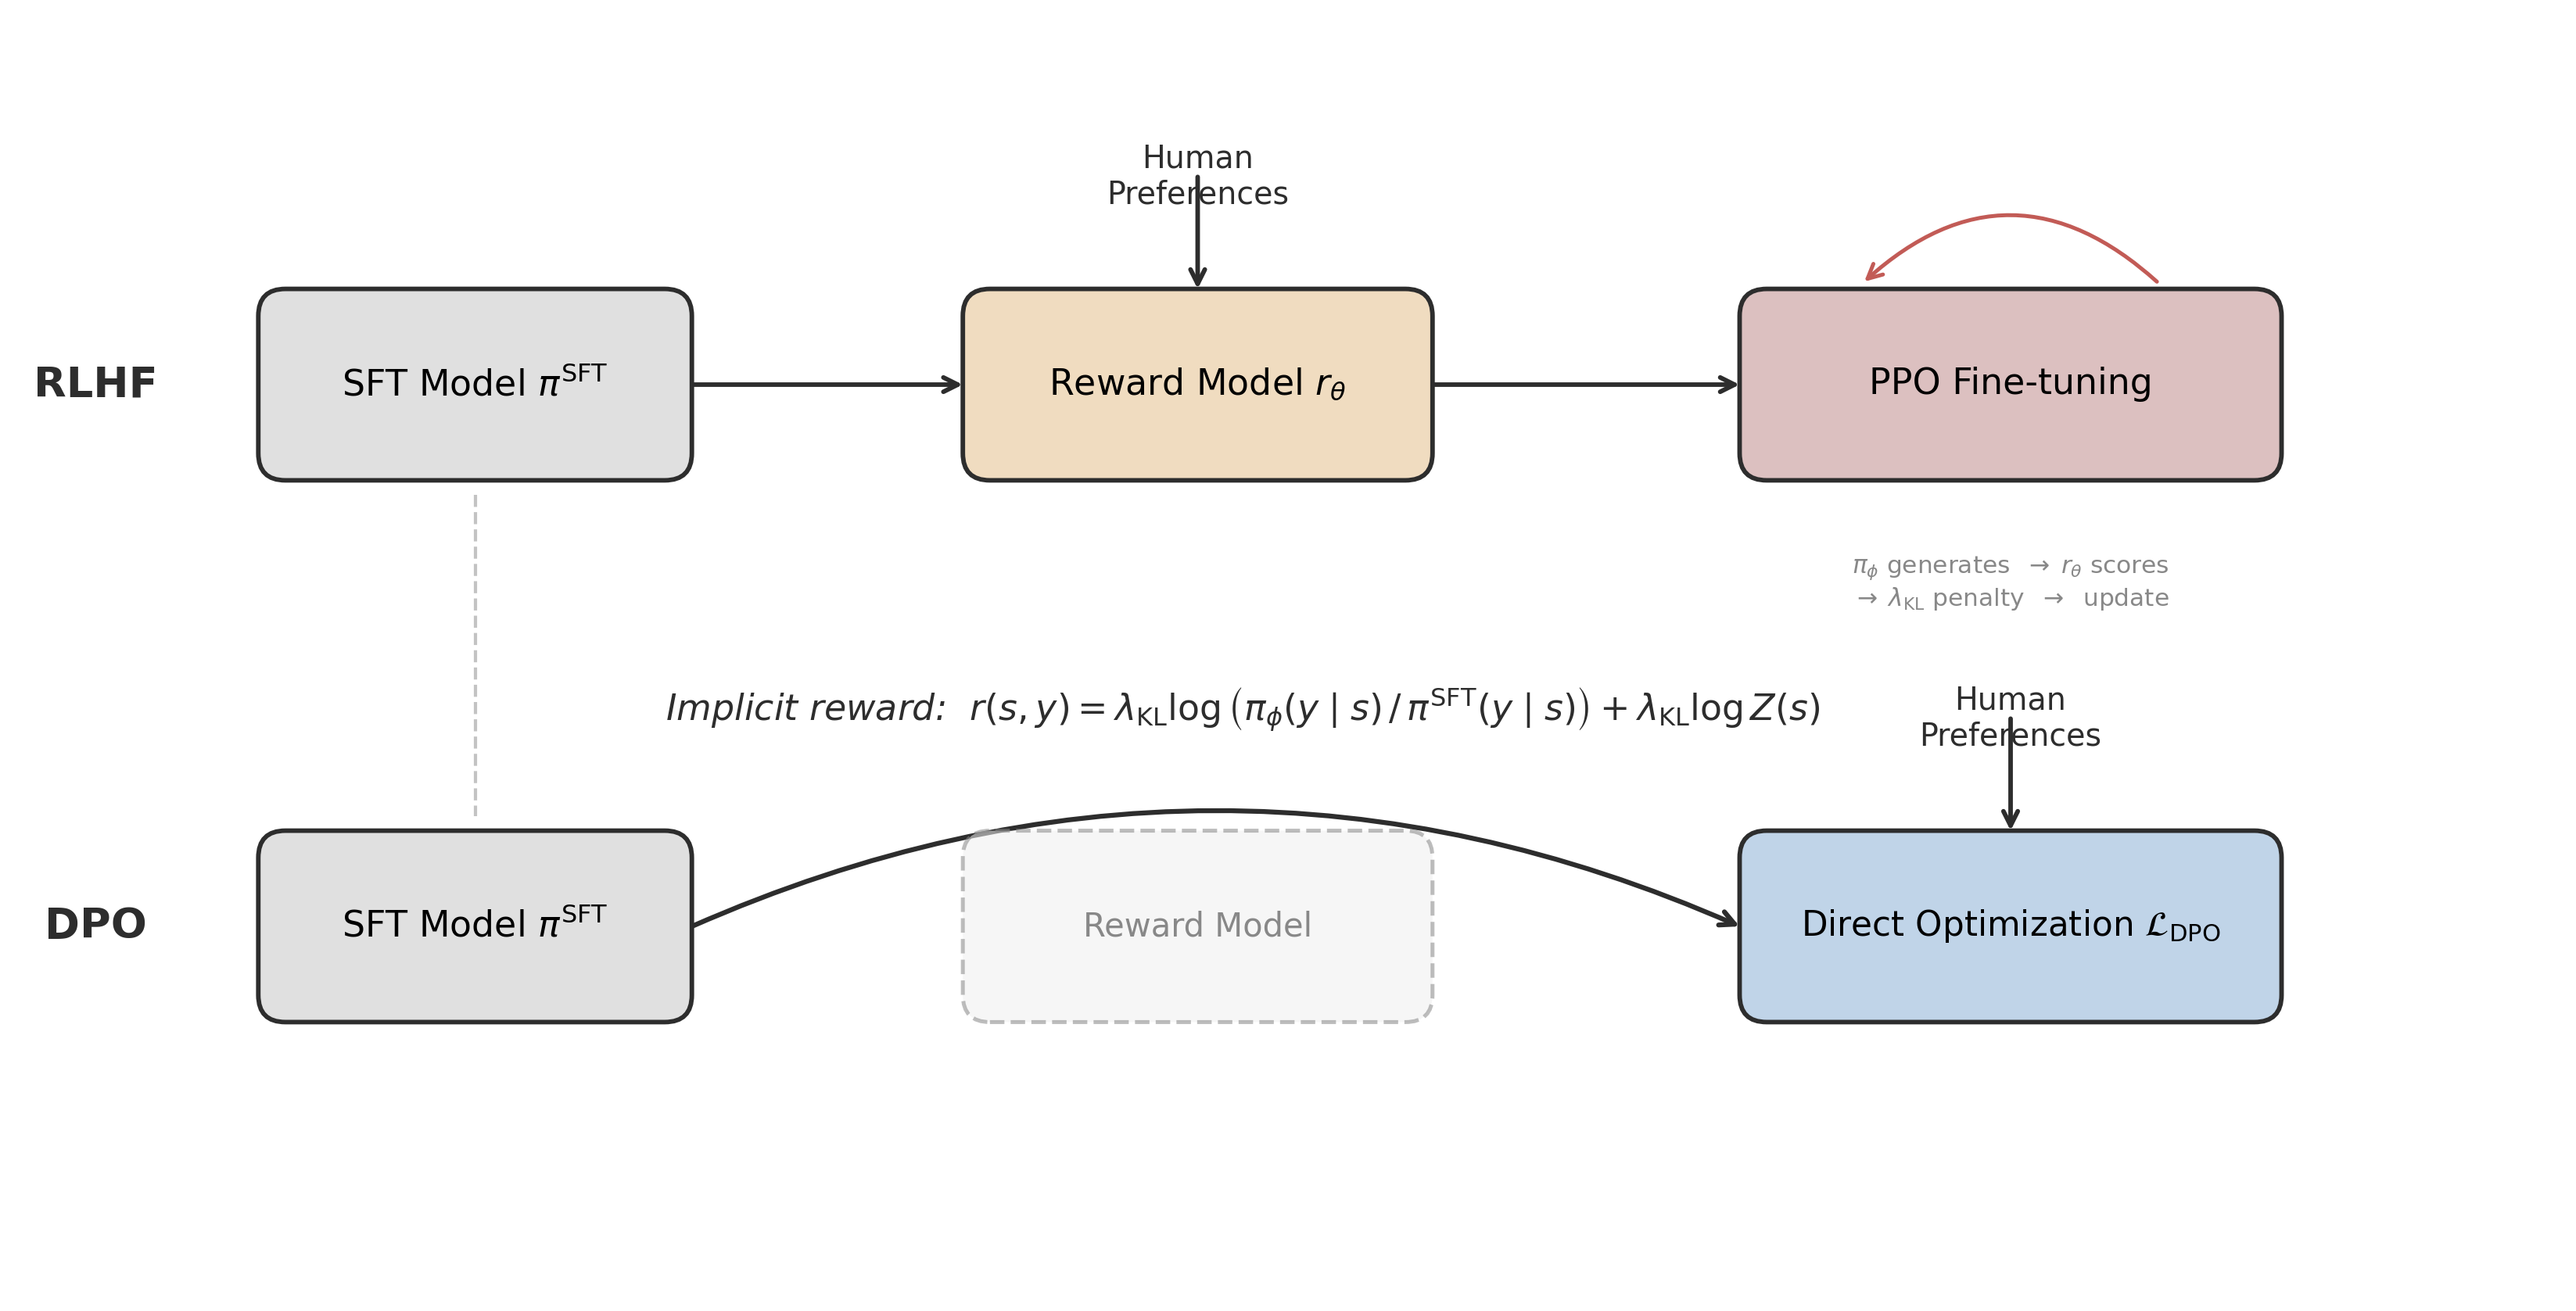
\includegraphics[width=\textwidth]{../ch09_rlhf/sims/rlhf_dpo_pipeline.png}
\caption[RLHF versus DPO pipelines]{\textbf{RLHF versus DPO pipelines.} Top row: the three-stage RLHF pipeline trains a reward model from human preferences, then uses PPO to fine-tune the policy with a KL penalty. Bottom row: DPO collapses the pipeline into a single supervised learning objective over preference pairs, eliminating the explicit reward model (ghosted box).}
\label{fig:rlhf_dpo_pipeline}
\end{figure}

\subsection{AI Alignment as Economics}
\label{sec:ai_alignment_economics}

RLHF turns alignment into an economics problem: elicit preferences, aggregate them across people, design incentives for truthful feedback, and interpret the learned object. The phrase ``alignment tax'' appears in the assistant-alignment literature as a warning that optimizing for helpfulness, harmlessness, and honesty can trade off against other capabilities \citep{askell2021general}; \citet{ouyang2022training} provide concrete InstructGPT evidence of benchmark regressions on tasks such as SQuAD, DROP, and HellaSwag. That evidence should not be read as a law of nature. It is an empirical frontier of a particular training recipe, model class, and evaluation set.

\subsubsection{Social Choice and Whose Preferences}

The central welfare question is whose preferences are being aligned to. If one reward model is trained on pooled labels from a non-representative group of contractors, the resulting policy optimizes an implicit aggregation rule, not society's preferences. Social choice supplies the vocabulary for this problem: alternatives, voters, ranking rules, impossibility theorems, strategic reports, minority protection, and interpersonal aggregation \citep{conitzer2024socialchoice,mishra2023socialchoice}. Distributional preference learning and axiomatic analyses show that standard BTL aggregation can encode Borda-like rules or fail desirable fairness and consistency conditions \citep{siththaranjan2024distributional,ge2024axioms}. Alternatives such as personalization, MaxMin-RLHF, Nash learning from human feedback, and maximal-lottery alignment make the aggregation rule more explicit, though some of these connections remain preprint-level rather than settled practice \citep{park2024heterogeneous,chakraborty2024maxmin,munos2023nash,maurarivero2025maximal}.

\subsubsection{Revealed Preference Tests of LLMs}

A related literature treats language models themselves as economic agents and asks whether their choices satisfy revealed-preference restrictions. Budget-allocation experiments, consumer-preference replications, moral-choice tasks, and Bayesian decision problems find that LLMs can look rational in some narrow domains and fragile in others \citep{chen2023rationalitygpt,golisingh2024preferences,seror2024moral,murawatrawat2025bayesian}. These tests are useful because they translate vague alignment claims into falsifiable restrictions, such as GARP consistency or proximity to a Bayes rule. But the results are prompt-, model-, version-, and domain-sensitive. They should be used as diagnostics of a trained system, not as evidence that an LLM has a stable utility function in the welfare-economics sense.

\subsubsection{Mechanism Design for Feedback}

Feedback is not passively observed; it is elicited through a mechanism. Labelers may be inattentive, strategic, ideologically motivated, or selected by the platform's contracting process. Mechanism design therefore enters before the reward model is trained. VCG-style fine-tuning formulations ask how to aggregate multiple reward models when participants can benefit from manipulating the training rule \citep{sun2024mechanism}. Strategyproof RLHF studies the same issue for preference reports, with a tradeoff between incentive compatibility and the quality of the final policy \citep{kleinebuening2025strategyproof}. Older peer-prediction mechanisms such as Bayesian truth serum and output-agreement methods show how payments can elicit truthful subjective signals when no ground truth is immediately observable \citep{prelec2004bayesian,miller2005eliciting}. For RLHF, this means the data-generating process is not a nuisance detail; it determines which preferences are observed and how costly truthful feedback is.

\subsubsection{Structural Identification}

Finally, preference optimization is not welfare analysis unless the learned reward has a structural interpretation. Bradley-Terry and DPO identify reward differences only through observed pairwise comparisons, up to normalizations and only on the covered comparison support. IRL identification results show that many rewards can rationalize the same behavior or preferences, and that entropy regularization, extra environments, or downstream invariance restrictions are needed to recover sharper objects \citep{cao2021identifiability,skalse2023invariance,knox2022preference}. Economically, the genealogy runs from McFadden logit choice \citep{mcfadden:1973}, through Rust-style dynamic discrete choice \citep{rust1994structural,rust1996numerical}, to maximum-entropy IRL \citep{Ziebart2008}, and finally to DPO's log-odds reparameterization \citep{rafailov2023direct}. Recent econometric work makes this bridge explicit, but still as an emerging working-paper literature rather than a settled textbook synthesis \citep{vanderlaan2025efficient}. The practical lesson is conservative: RLHF can produce useful policies, but the reward object is partially identified, aggregation-dependent, and limited by the offline support of the comparison data.

\subsection{Simulation Study: Preference Learning in Job Search}

A worker searches for jobs in a labor market with compensating differentials, following a McCall (1970)-style search model. Wages are measured in thousands and take values $w \in \{20,28,38,50,65,82,100,125\}$, while amenities take values $z \in \{0, 1, \ldots, 6\}$ and capture commute quality, flexibility, and job security. The state space has 112 states: 56 searching states in which the worker observes a pending offer $(w_i, z_j)$ and decides to accept or reject, plus 56 employed states $(w_i, z_j)$ in which the worker decides to stay or quit. The offer distribution exhibits compensating differentials, with wage rank and amenity rank negatively correlated ($\rho = -0.74$): high-wage offers cluster with low amenities and vice versa. The worker's true per-period utility is $u(w, z) = \alpha \log(w) + (1 - \alpha) z$ with $\alpha = 0.6$, but this function is unobserved; the worker can only compare career trajectories (``I prefer path A to path B''), exactly as in stated-preference surveys in labor economics. While searching, the worker receives the unemployment benefit $u_b = \alpha \log(b)$ where $b = 28$. Layoffs occur with probability $p = 0.05$ per period, and the discount factor is $\gamma = 0.95$. Dynamic programming gives $V^*(s_0) = 74.13$; the optimal policy accepts 25 of 56 offer types and stays employed at 25 of 56 job types. Preference data is generated by rolling out a uniform random policy from a random searching state. Each rollout produces a career segment of $L = 15$ periods recording states and actions. For each of $K$ comparisons, two independent career segments are generated; the segment with higher cumulative discounted utility under the true (unobserved) utility function is labeled as preferred via the Bradley-Terry model. Figure~\ref{fig:search_env} shows the optimal accept/reject and stay/quit boundaries.

\begin{figure}[htbp]
\centering
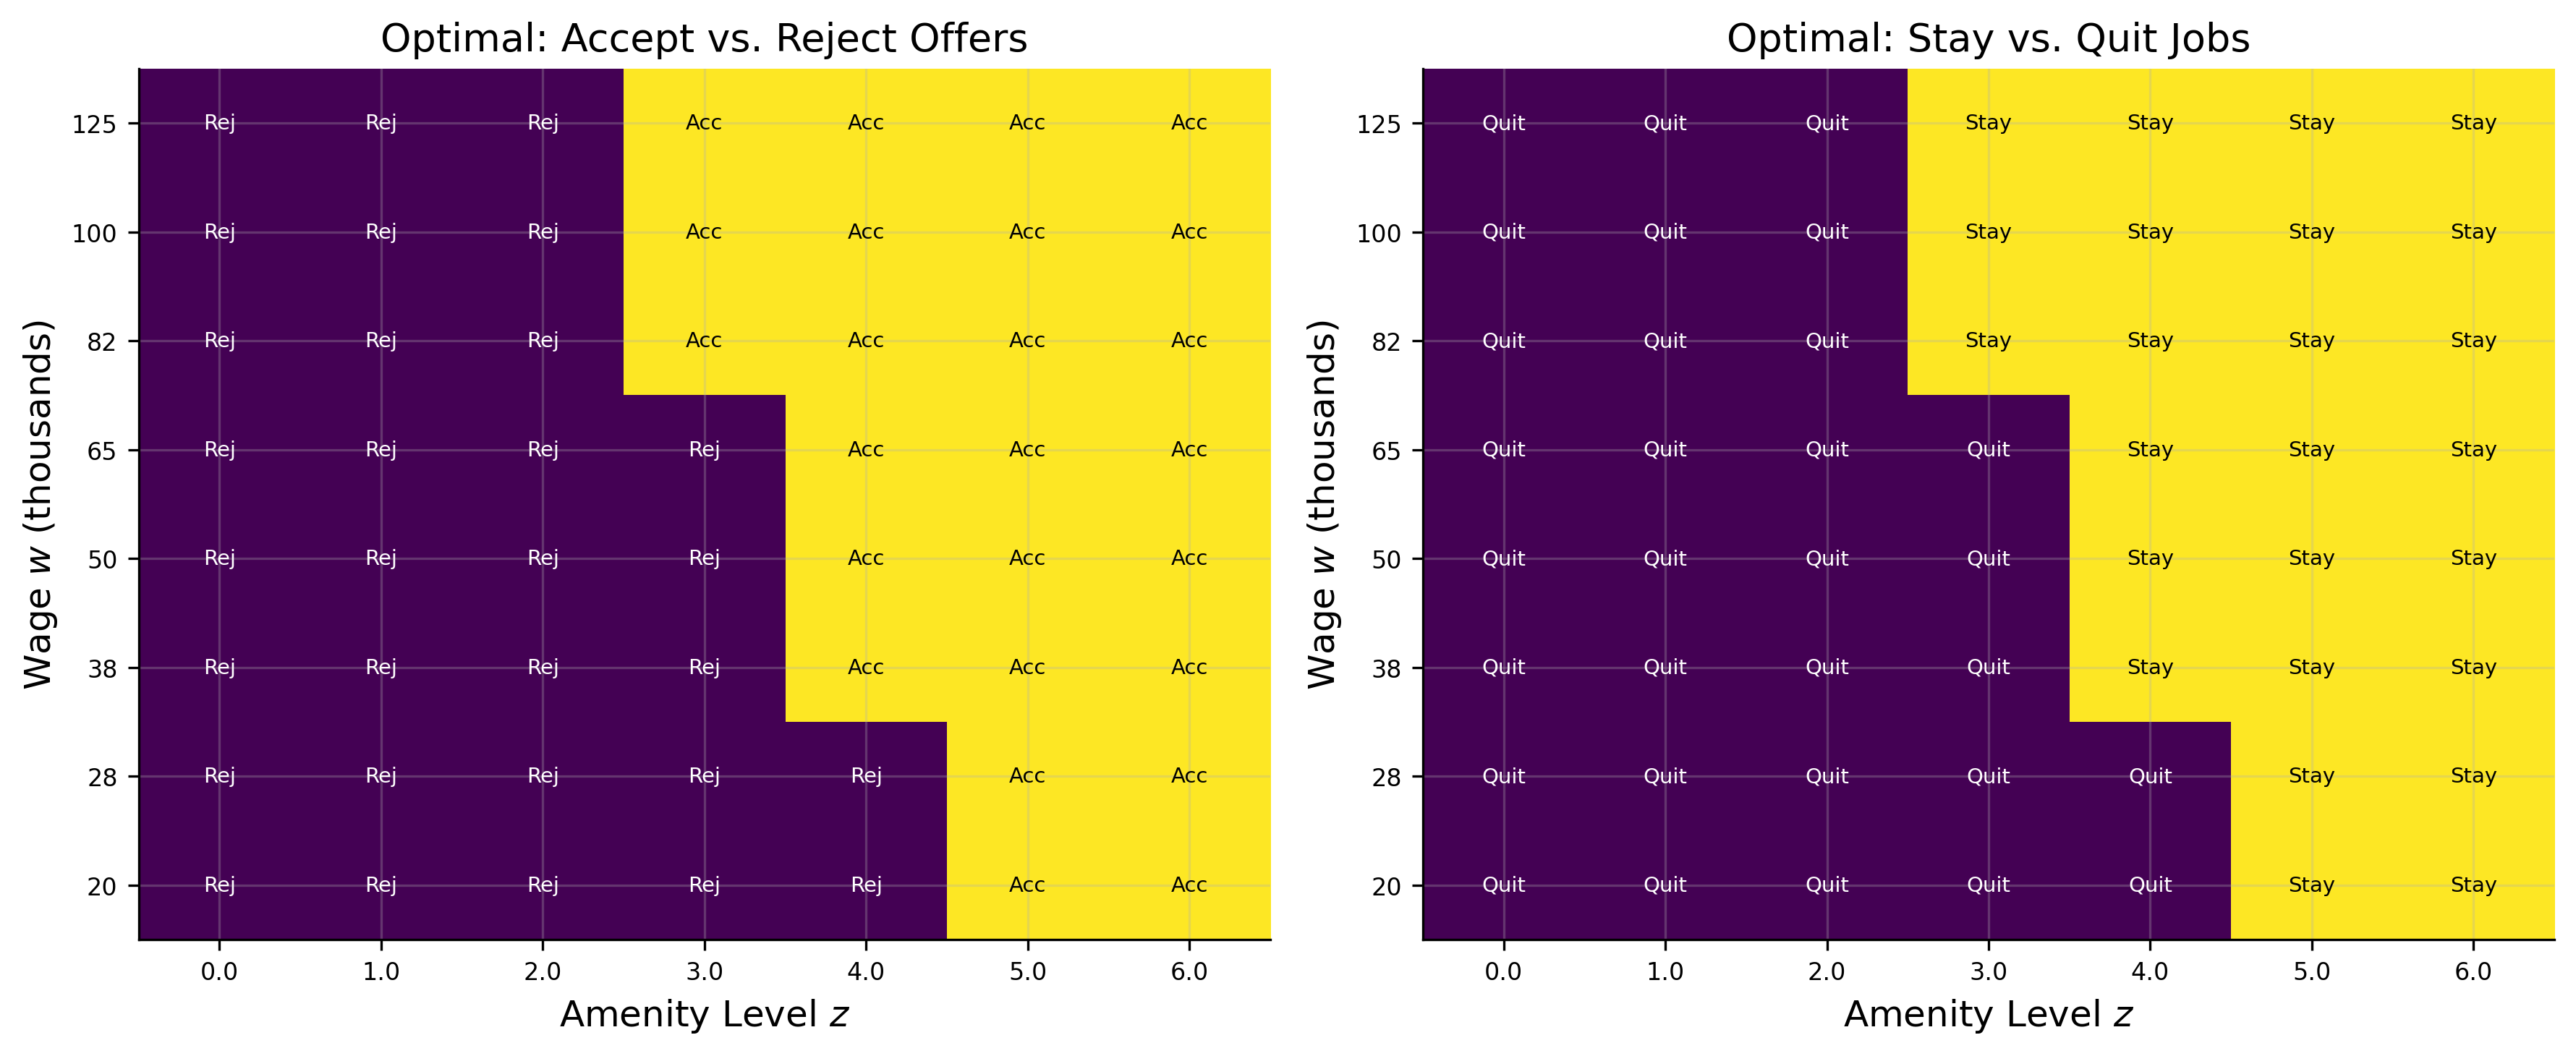
\includegraphics[width=0.85\textwidth]{../ch09_rlhf/sims/job_search_env.png}
\caption[Optimal accept/reject and stay/quit boundaries in wage-amenity space]{\textbf{Optimal accept/reject and stay/quit boundaries in wage-amenity space.} Left: the optimal accept/reject boundary for searching states. Right: the optimal stay/quit boundary for employed states. Both boundaries cut diagonally, reflecting the tradeoff between wage and amenity quality under compensating differentials.}
\label{fig:search_env}
\end{figure}

Six methods are compared across $K \in \{25, 50, 100, 200, 500, 1{,}000, 2{,}000, 5{,}000\}$, averaged over 30 seeds. The neural network RLHF reward model is a two-layer MLP trained by Bradley-Terry MLE on the $K$ segment pairs; per-transition rewards are discount-weighted and summed to obtain a segment score, and the resulting 112-state reward table is solved by value iteration.\footnote{The neural network has 4 inputs (normalized log-wage, normalized amenity, employment indicator, action), 32 hidden units per layer, and $\sim$1{,}200 parameters. The logistic loss from Equation~(\ref{eq:rlhf_loss}) is applied to discount-weighted segment reward sums. The network parameterises $r_\theta(s, a)$, but the table handed to value iteration averages over actions to give $\bar{r}(s) = \tfrac{1}{2}(r_\theta(s, 0) + r_\theta(s, 1))$; this is harmless here because the true per-period reward in this environment is action-independent (actions affect only the next-state transition), so the Bradley-Terry MLE has no incentive to fit action-dependent payoffs.} The correctly specified structural model parameterizes utility as $\hat{u} = \hat{\alpha} \log(w) + (1 - \hat{\alpha}) z$, estimating the single parameter $\hat{\alpha}$ via Bradley-Terry MLE, then solves the MDP. The misspecified model uses $\hat{u} = \hat{\alpha} \log(w) + (1 - \hat{\alpha}) \bar{z}$, where $\bar{z} = 3$ is the mean amenity level; this model ignores amenity variation across jobs, treating all amenities as identical. DPO trains a tabular softmax policy directly from trajectory comparisons, bypassing reward modeling entirely.\footnote{DPO uses 112 logit parameters $\phi_s$, one per state, trained via the DPO loss (Equation~\ref{eq:dpo_loss}) with Adam optimization over a sweep of $\lambda_{KL} \in \{0.01, 0.05, 0.1, 0.5, 1.0, 5.0\}$, selecting the $\lambda_{KL}$ that minimizes training loss. The reference policy is uniform: $\pi^{SFT}(a|s) = 0.5$. To match the LLM setup where both completions condition on the same prompt, DPO comparison pairs start from the same initial state.} Tabular Q-learning ($10{,}000$ episodes, $\varepsilon = 0.15$, learning rate $0.1$) and exact DP provide scalar-reward baselines. All four preference methods receive identical comparison data per seed; DPO receives a same-state variant generated from the same seed.

\begin{figure}[htbp]
\centering
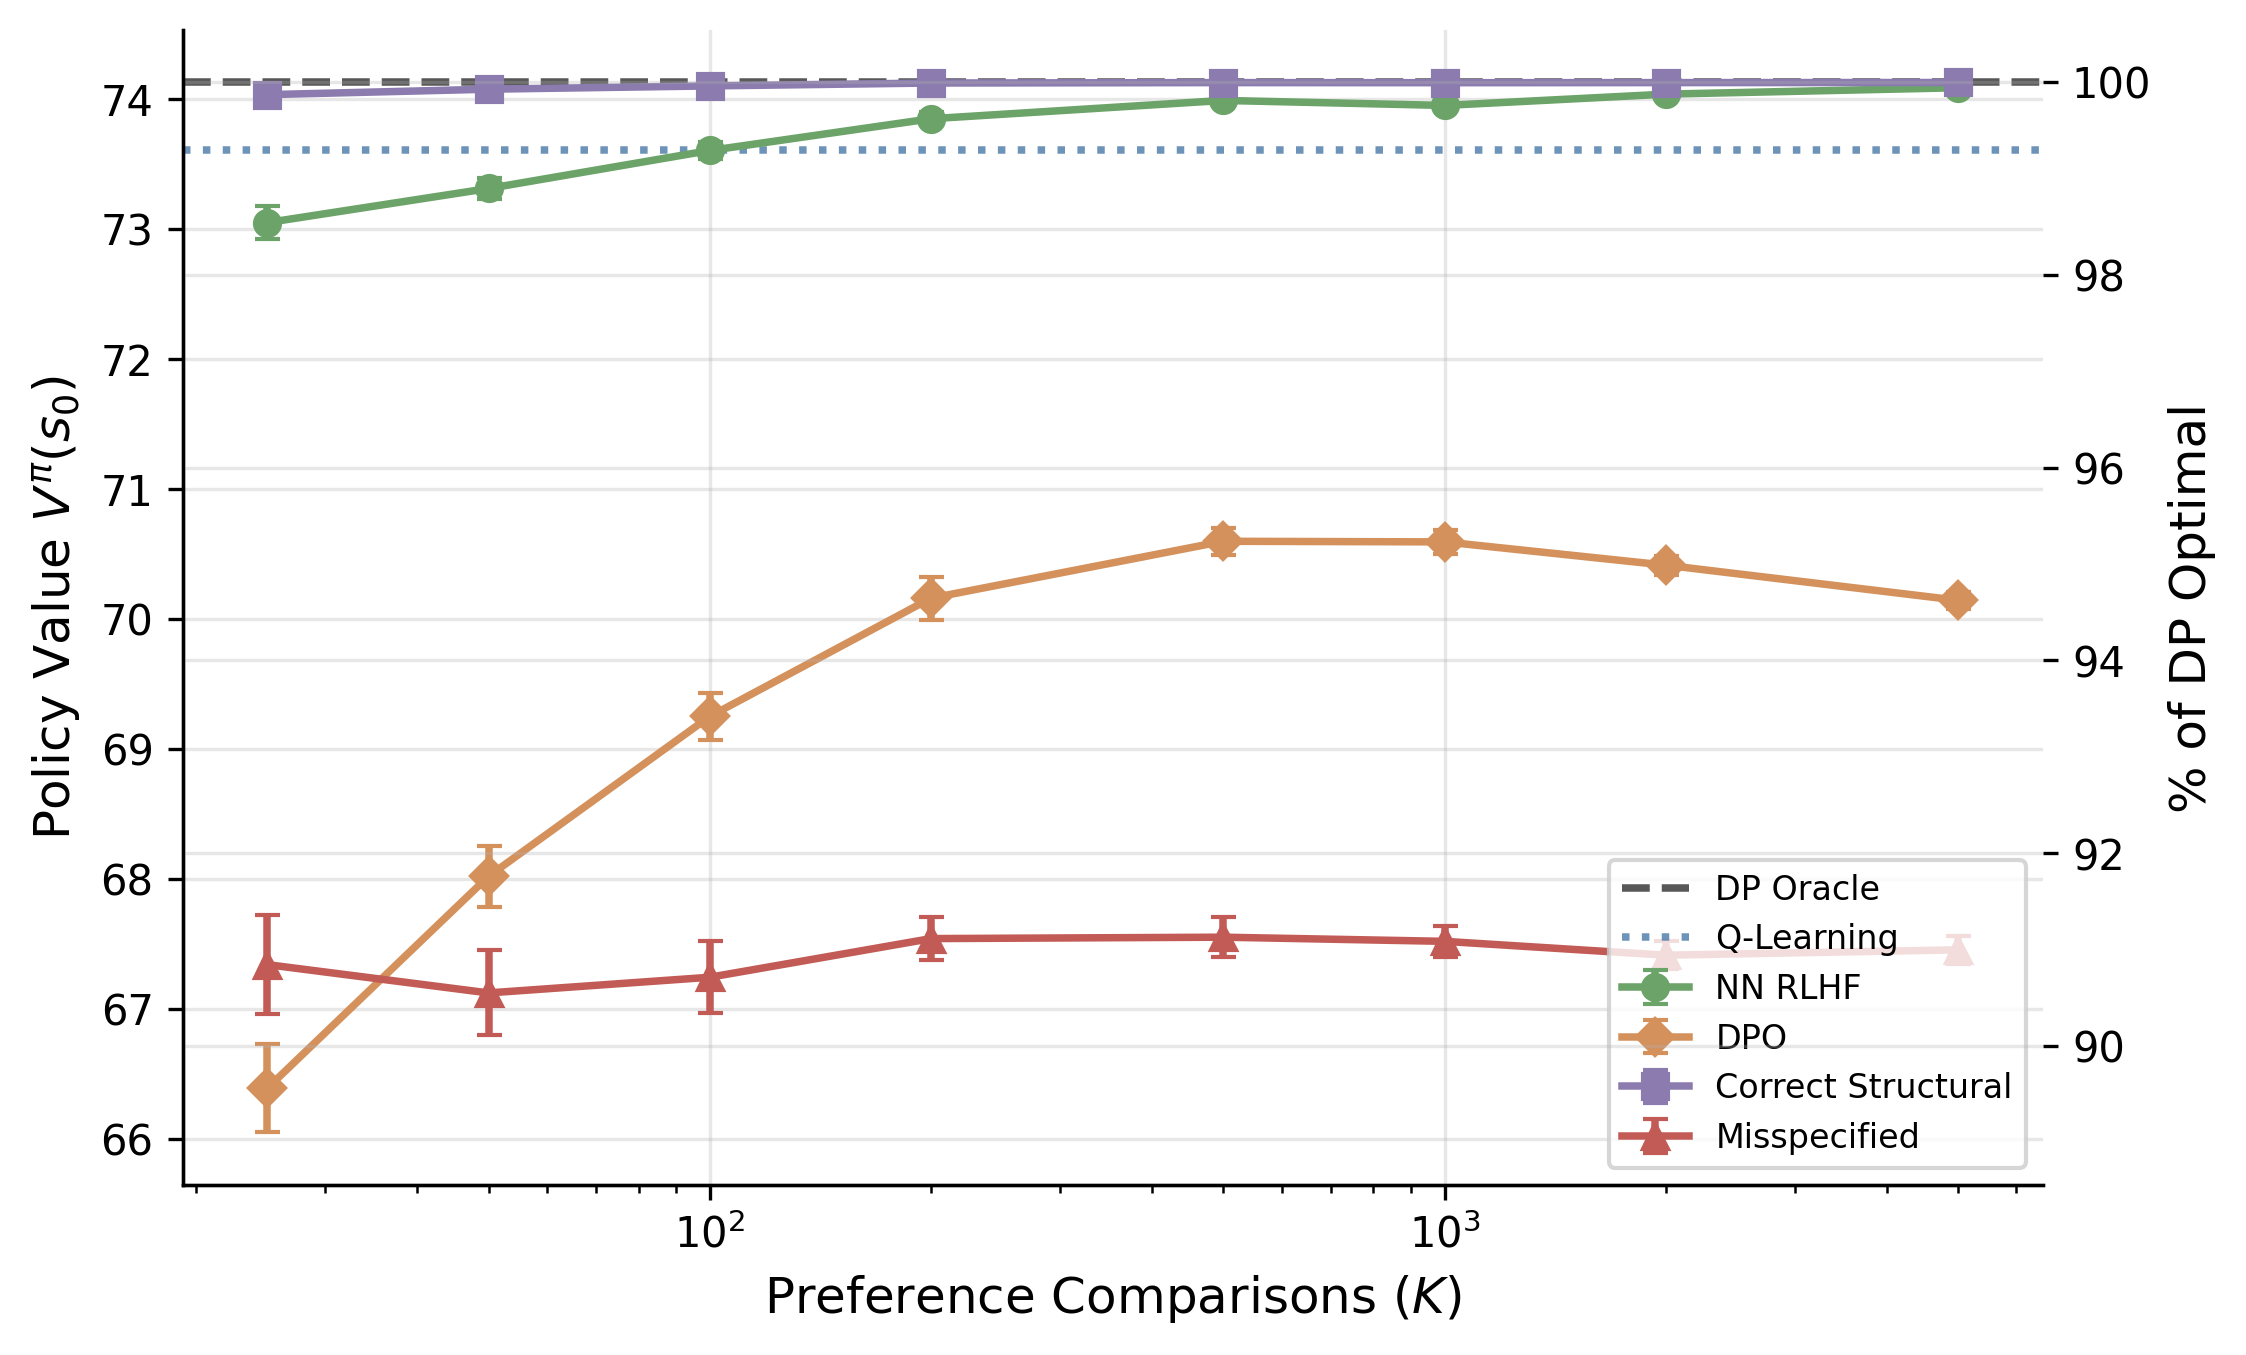
\includegraphics[width=0.7\textwidth]{../ch09_rlhf/sims/job_search_sample_complexity.png}
\caption[Policy value versus number of preference comparisons $K$ for all six methods]{\textbf{Policy value $V^\pi(s_0)$ versus number of preference comparisons $K$ for all six methods (30 seeds, $L = 15$).} The right axis shows the percentage of DP-optimal value.}
\label{fig:preference_sample}
\end{figure}

Figure~\ref{fig:preference_sample} reports the main results. Three findings stand out. First, the correctly specified structural model dominates: even at $K = 25$ it achieves 99.9\% of DP-optimal, illustrating the power of correct specification when the model has a single free parameter. Second, the neural network converges more slowly but reaches 99.9\% by $K = 5{,}000$, reflecting the higher sample complexity of a flexible model relative to a one-parameter structural specification. Third, DPO plateaus at approximately 95\% by $K = 500$ and does not improve further.\footnote{DPO learns only from $(s,a)$ pairs visited in training trajectories generated by the random behavioral policy. It cannot propagate value to undervisited states the way value iteration does after learning a reward model, so states poorly covered by the behavioral policy remain suboptimal regardless of $K$.} This plateau is qualitatively different from the gridworld failure ($-118\%$): DPO recovers a reasonable policy, but the gap does not close with additional data.\footnote{DPO fails catastrophically in gridworld because transitions are stochastic (10\% slip probability) and rewards are transition-dependent. The same $(s,a)$ pair yields different rewards depending on whether the agent slipped, so the DPO loss conflates policy quality with transition luck. In the job search model, accept/reject deterministically changes employment status, and only the 5\% layoff probability introduces stochastic transitions.} The misspecified constant-amenity model plateaus at 91\% regardless of $K$, because additional preference data cannot correct the omitted variable.

\begin{table}[htbp]
\centering
\caption[Diagnostics at $K = 5{,}000$: policy agreement with $\pi^*$, value-function correlation, and mean accepted wage and amenity for each method]{\textbf{Diagnostics at $K = 5{,}000$ (single seed): policy agreement with $\pi^*$, value-function correlation, and mean accepted wage and amenity for each method.}}
\label{tab:preference_diagnostics}
\input{../ch09_rlhf/sims/job_search_diagnostics.tex}
\end{table}

Table~\ref{tab:preference_diagnostics} provides state-level diagnostics at $K = 5{,}000$. The structural model and neural network achieve near-perfect policy agreement with $\pi^*$ (100\% and 96\% respectively). DPO agrees on only 57\% of states with value-function correlation 0.78, systematically underselecting on both wage and amenity dimensions.\footnote{DPO's mean accepted amenity of 3.4 parallels the misspecified structural model's 3.0, though the mechanisms differ: the misspecified model ignores amenity variation by construction, while DPO underweights amenities because the random behavioral policy underrepresents high-amenity employed states in the training data.} The misspecified model agrees on 50\%, with disagreements concentrated where amenity variation matters.\footnote{An online versus offline ablation for the neural network at $K = 1{,}000$ (20 seeds) shows comparable performance: online $73.92 \pm 0.05$, offline $73.99 \pm 0.03$ ($p = 0.09$). The random behavioral policy already provides diverse career trajectories covering the full wage-amenity space.}

\begin{figure}[htbp]
\centering
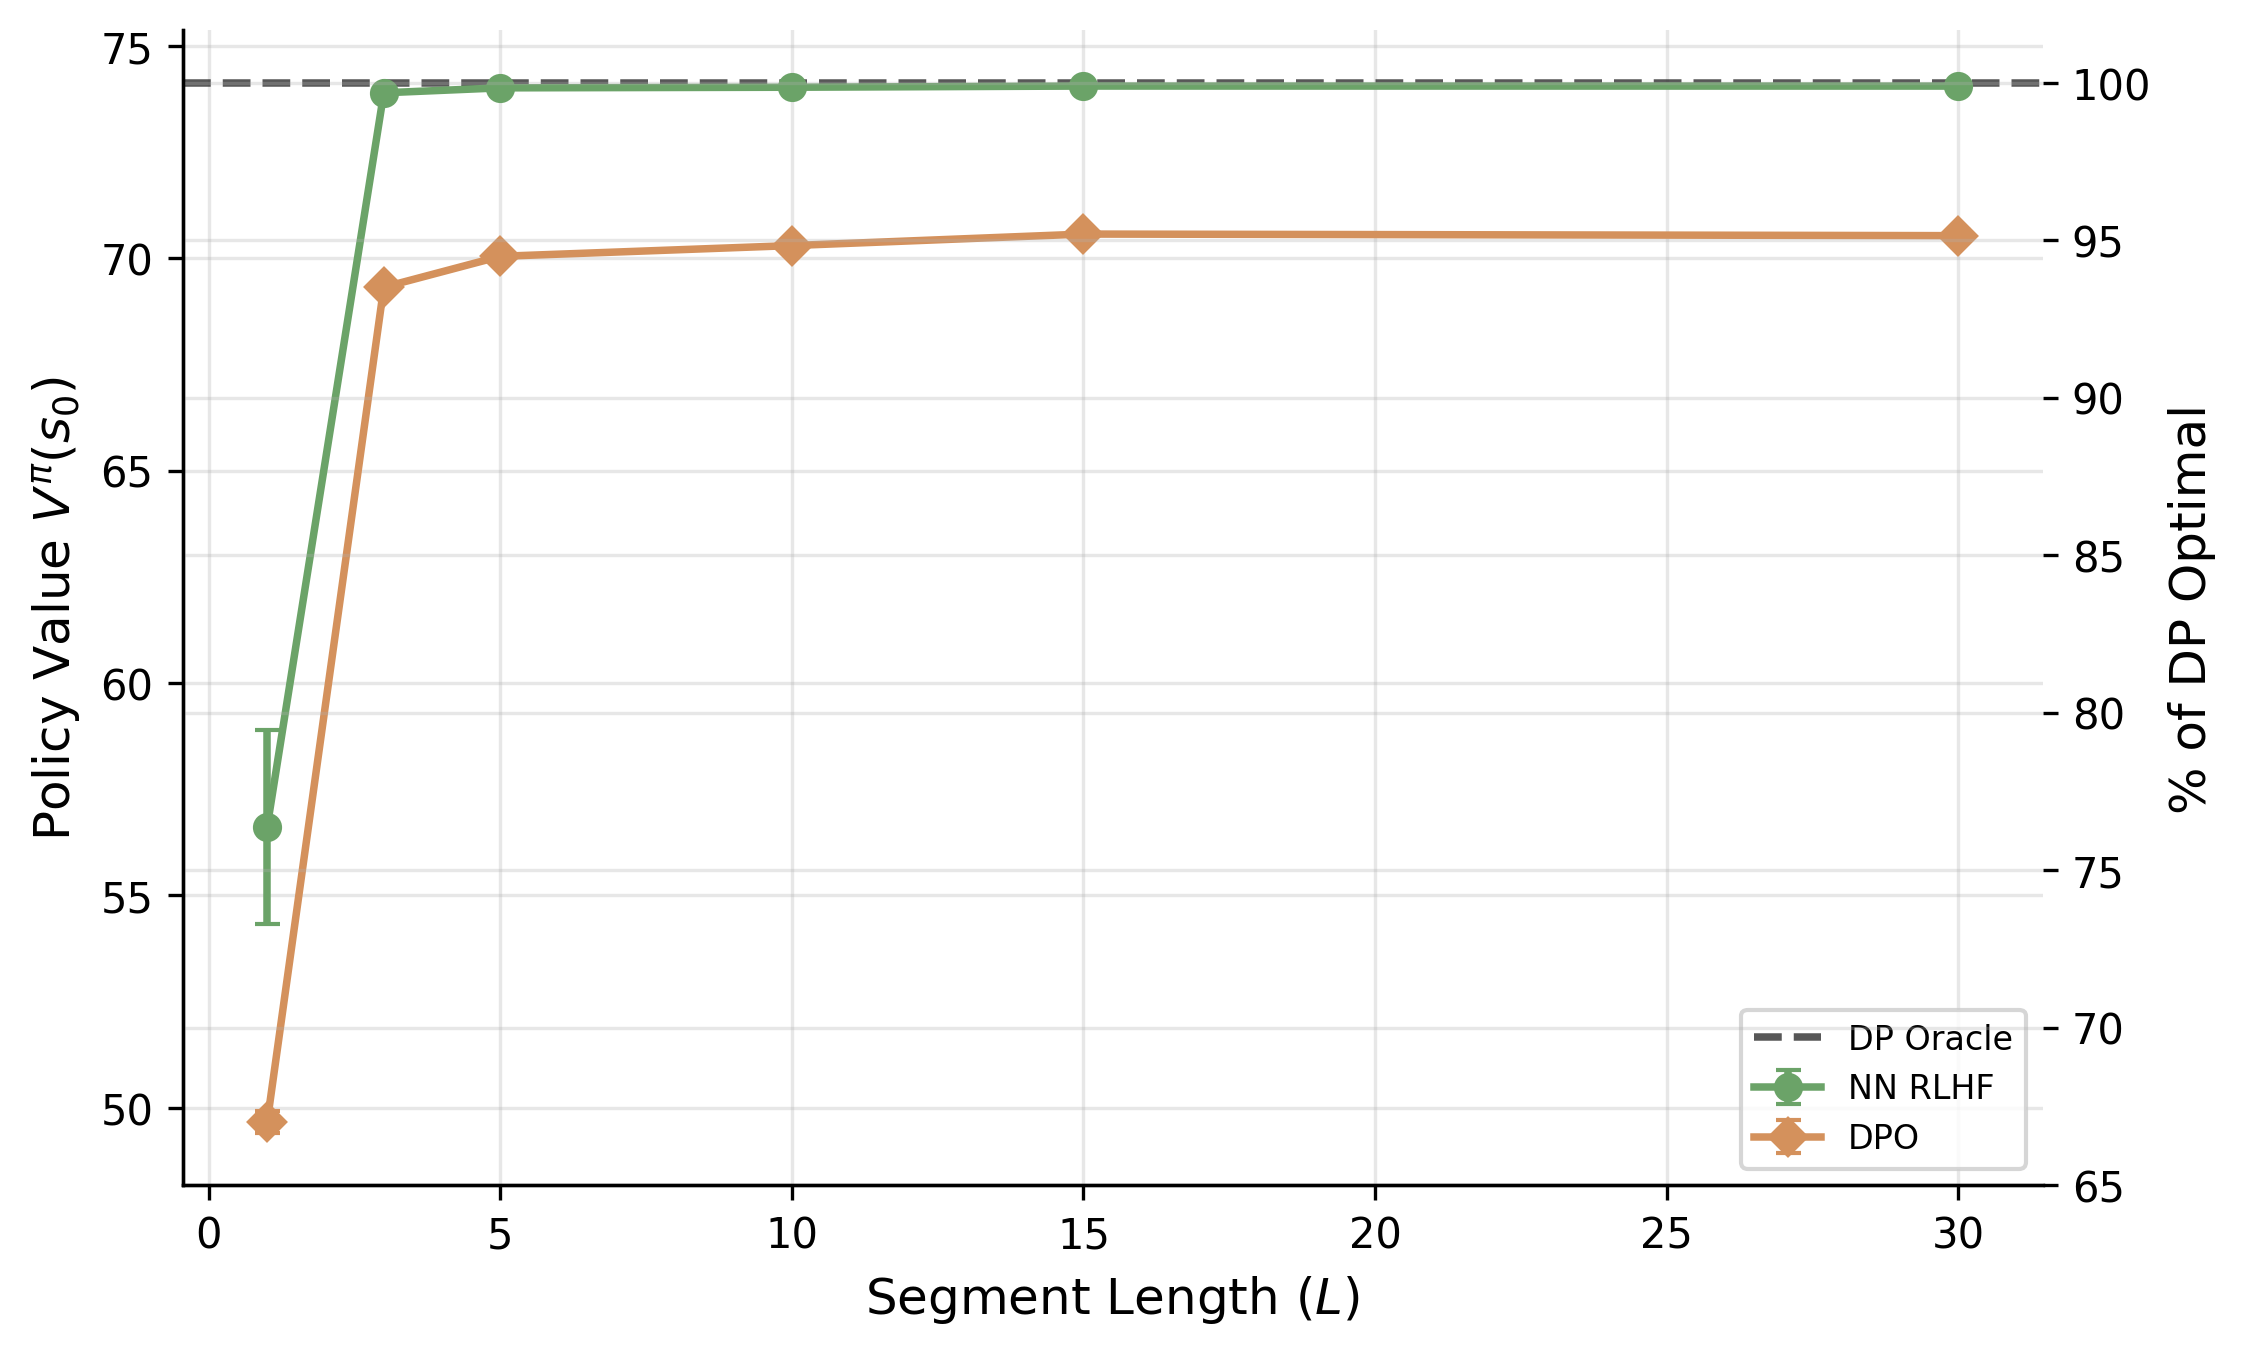
\includegraphics[width=0.7\textwidth]{../ch09_rlhf/sims/job_search_horizon.png}
\caption[Policy value versus segment length $L$ at $K = 2{,}000$ for the neural network and DPO]{\textbf{Policy value $V^\pi(s_0)$ versus segment length $L$ at $K = 2{,}000$ for the neural network and DPO (20 seeds).} The right axis shows the percentage of DP-optimal value.}
\label{fig:preference_horizon}
\end{figure}

Figure~\ref{fig:preference_horizon} reports the segment length ablation at $K = 2{,}000$. At $L = 1$, both methods perform poorly because single-step comparisons carry minimal information about long-run value. The neural network recovers rapidly (by $L = 3$) because the reward model aggregates per-transition estimates over longer segments and value iteration propagates them through the full transition structure; DPO improves monotonically but plateaus at its $\sim$95\% ceiling, as it must learn the policy directly from trajectory comparisons without access to the transition model.

Two-stage RLHF separates preference estimation (a static econometric problem) from dynamic programming (which exploits the known transition model); DPO conflates the two and forfeits the transition structure that structural modelers typically have access to.\footnote{This advantage is specific to settings where the transition model is known or estimable; in domains without a tractable transition model, DPO's single-stage approach avoids compounding errors from reward model estimation.} The DPO plateau in the job-search study is the computational version of the identification point above. More comparisons tighten the empirical binary choice model on the support of observed trajectories, but they do not reveal counterfactual value in poorly covered states, nor do they identify a welfare object independent of the aggregation rule used to construct the labels.
